\chapter{PaaS Management}\label{paas-management}

This chapter describes the stack around a container-based production
environment, and how applications could take advantage on it.

\begin{figure}[htbp]
\centering
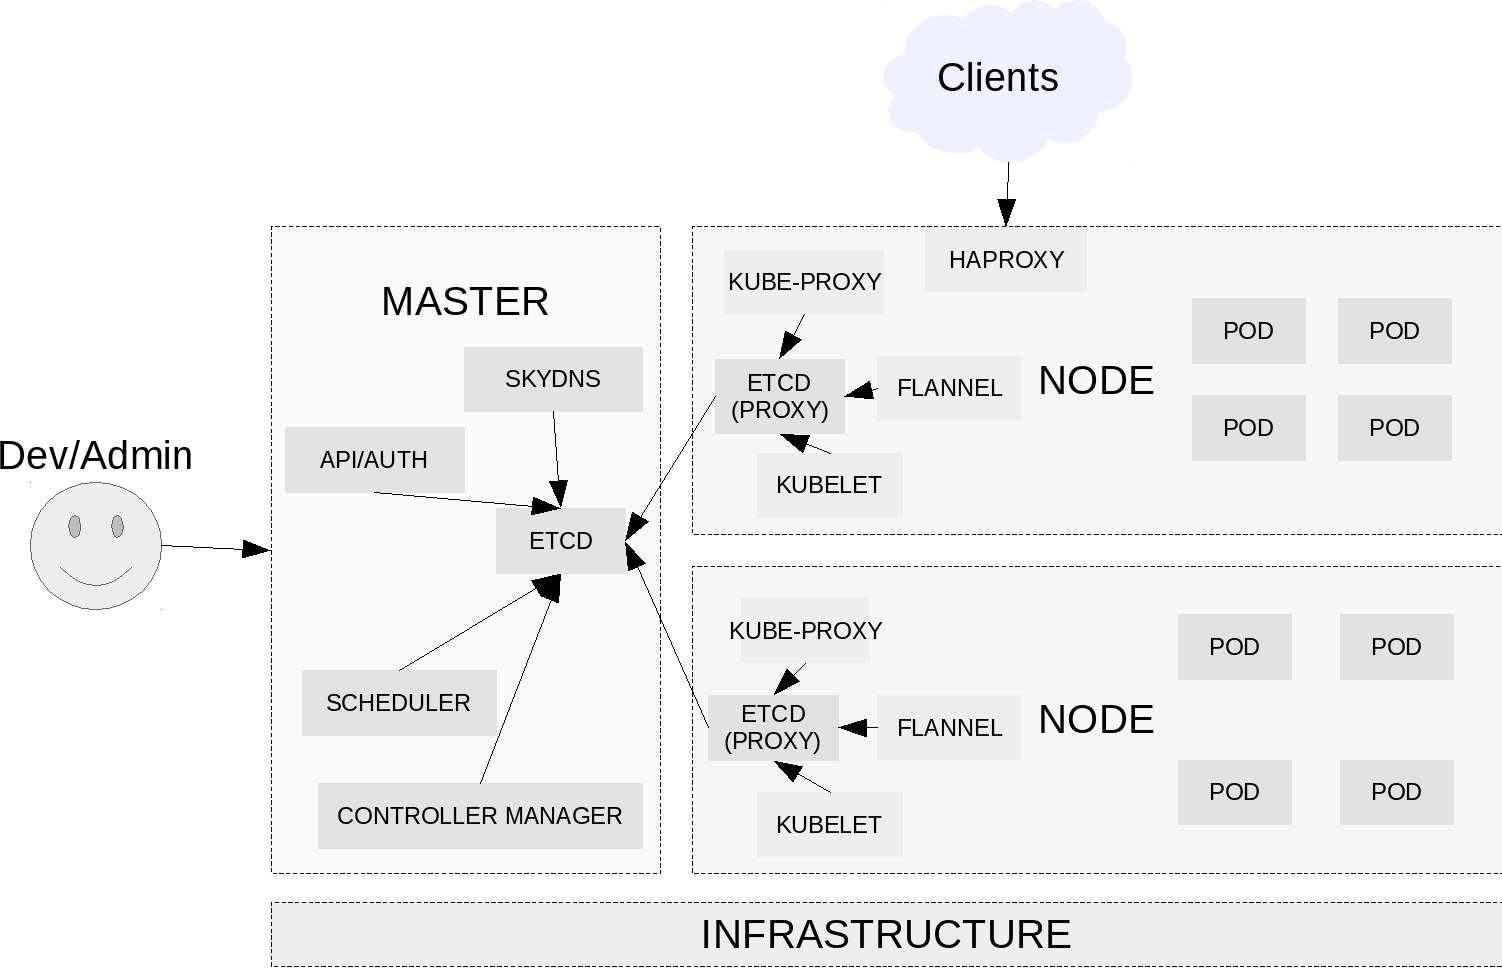
\includegraphics{media/ch5-overview.png}
\caption{Cluster Overview}
\end{figure}

\section{The Container Cluster's
Core}\label{the-container-clusters-core}

The basic building block for deploying containerized application remain
the operating system. But as all the application dependencies are
demanded to containers, there is only need basic functionality, without
package manager and other features of a traditional OS.

\emph{CoreOS} was announced in summer 2013 as a Gentoo-based GNU/Linux
distribution for deploying containers in a clustered environment. CoreOS
occupies few memory and comes with \emph{SystemD}, \emph{Docker} and
tools for distributed cluster environments.

\emph{SystemD} is the de-facto standard in GNU/Linux distribution as
init daemon. It made easy to daemonize processes and has advanced
features such as parallelization and socket activation, so the SSH
daemon is stopped by default, and it will be started only after an
incoming request, in order to save memory.

\emph{Etcd} is a distributed key-value database which represent the core
of the cluster since it has been used for inter-host communication by
all components. It could be used as master-slave (as in this project) or
also in high availability with a simply Raft-based algorithm for master
election. Etcd is the \emph{cluster database}, so it's really a core
component.

\emph{Fleet} provides a distributed init system, extending SystemD
functionality from host-level to cluster-level. This component has not
been used but it's useful for bootstrap the above stack, since it could
deploy SystemD services in all connected hosts.

\emph{Flannel} has been development for providing a subnet mask to every
host, enabling an overlay network for container inter-host
communication. It's a requisites of Kubernetes networking model. At the
boot, Flannel set the network data into etcd under \texttt{/coreos.io}
key.

CoreOS development is organized in 3 channels: alpha, beta and stable.
Alpha is generally release once a week and includes new software, while
stable it's more suitable for production.

Alternatives are Rancher OS (http://rancher.com/rancher-os/), Atomic
(http://www.projectatomic.io/) by Red Hat and Ubuntu Snappy
(http://www.ubuntu.com/cloud/tools/snappy) by Canonical.

\section{Microservices Scaling and
Orchestration}\label{microservices-scaling-and-orchestration}

Kubernetes (http://kubernetes.io/) has been announced at Google I/O in
June 2014, it's a cluster management system, a framework for container
scheduling and orchestration in a clustered environment. It fits a level
on top of an operating system like CoreOS.

Kubernetes has been developed by the same engineers developed the actual
Google infrastructure, and take advantace of that experience.

Core concepts of Kubernetes are:

\begin{itemize}
\itemsep1pt\parskip0pt\parsep0pt
\item
  \texttt{node} is a single node of the cluster
\item
  \texttt{pod} is a set of one or more containers, thinked as a single
  logic unit
\item
  \texttt{replicationController} is concerned about guarantee the
  correct numbers of replicas of a pod
\item
  \texttt{service} provides a virtual IP that load balance to a set of
  pods
\end{itemize}

\begin{figure}[htbp]
\centering
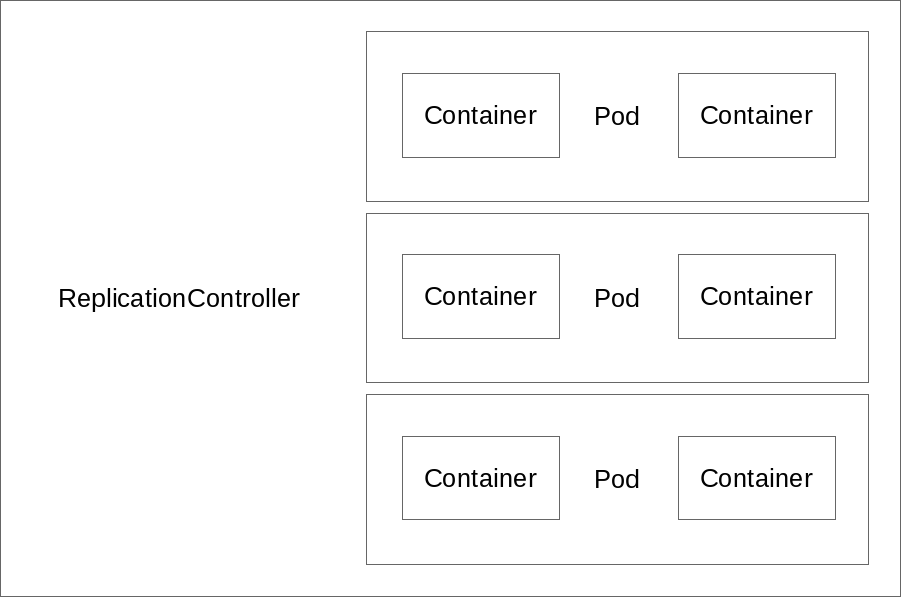
\includegraphics{media/ch5-pods-rcs.png}
\caption{Pods and Replication Controllers}
\end{figure}

\begin{figure}[htbp]
\centering
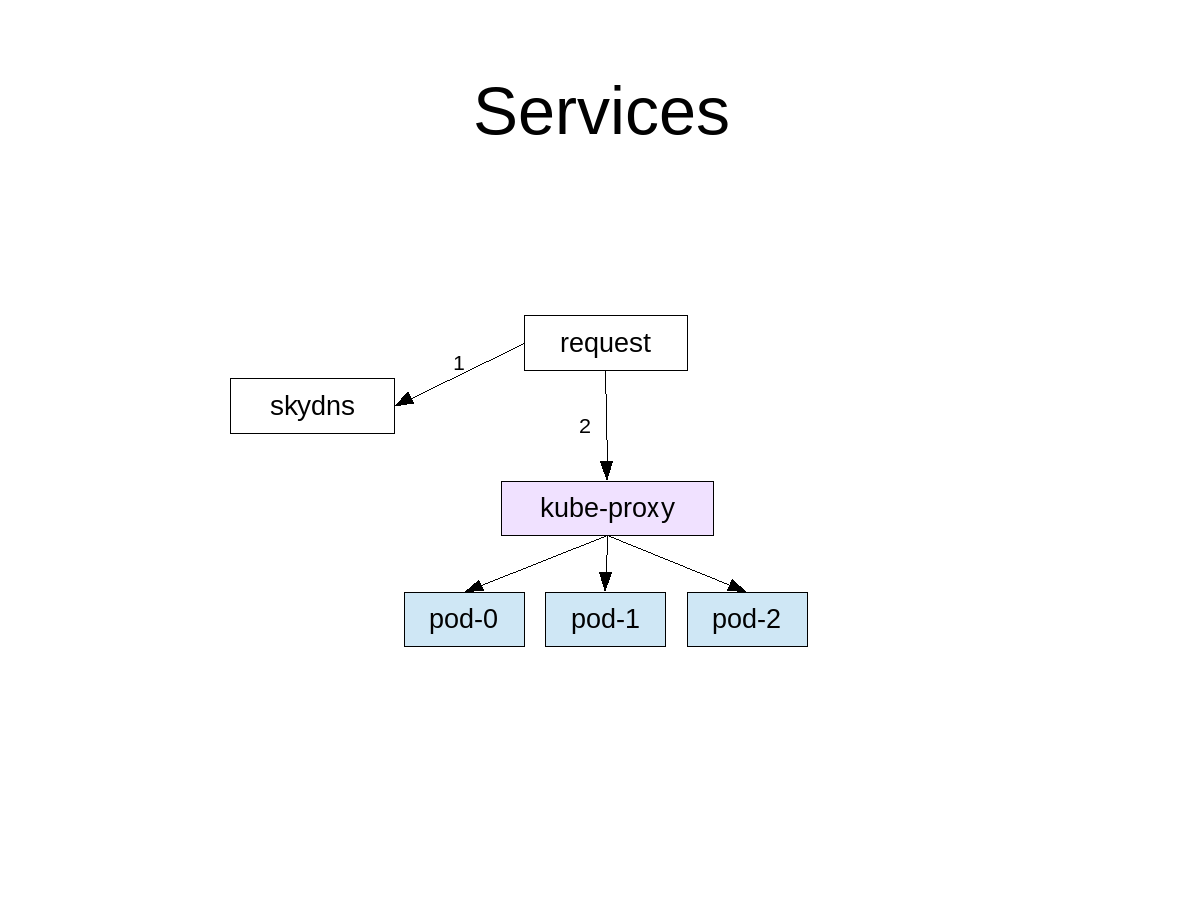
\includegraphics{media/ch5-services.png}
\caption{Scaling Pods with Kubernetes services}
\end{figure}

Components of Kubernetes are divided in master and node. The Master ones
are:

\begin{itemize}
\itemsep1pt\parskip0pt\parsep0pt
\item
  \emph{API Server} validates and configures the data for pods,
  services, and replication contorllers
\item
  \emph{Controller Manager} watches etcd for changes to replication
  controller and then uses the API to enforce the desired state
\item
  \emph{Scheduler} schedule the pods into nodes
\end{itemize}

Instead the components of Kubernetes Node are:

\begin{itemize}
\itemsep1pt\parskip0pt\parsep0pt
\item
  \emph{Kubelet} updates the node as specified in local etcd
\item
  \emph{Proxy} manages the services defined in the API on that node
\end{itemize}

Kubernetes stores the data about \texttt{node}s, \texttt{pod}s,
\texttt{replicationController}s, \texttt{service}s and other objects in
etcd under \texttt{/kubernetes.io} key.

These concepts could be summarized in the following diagram:

\begin{figure}[htbp]
\centering
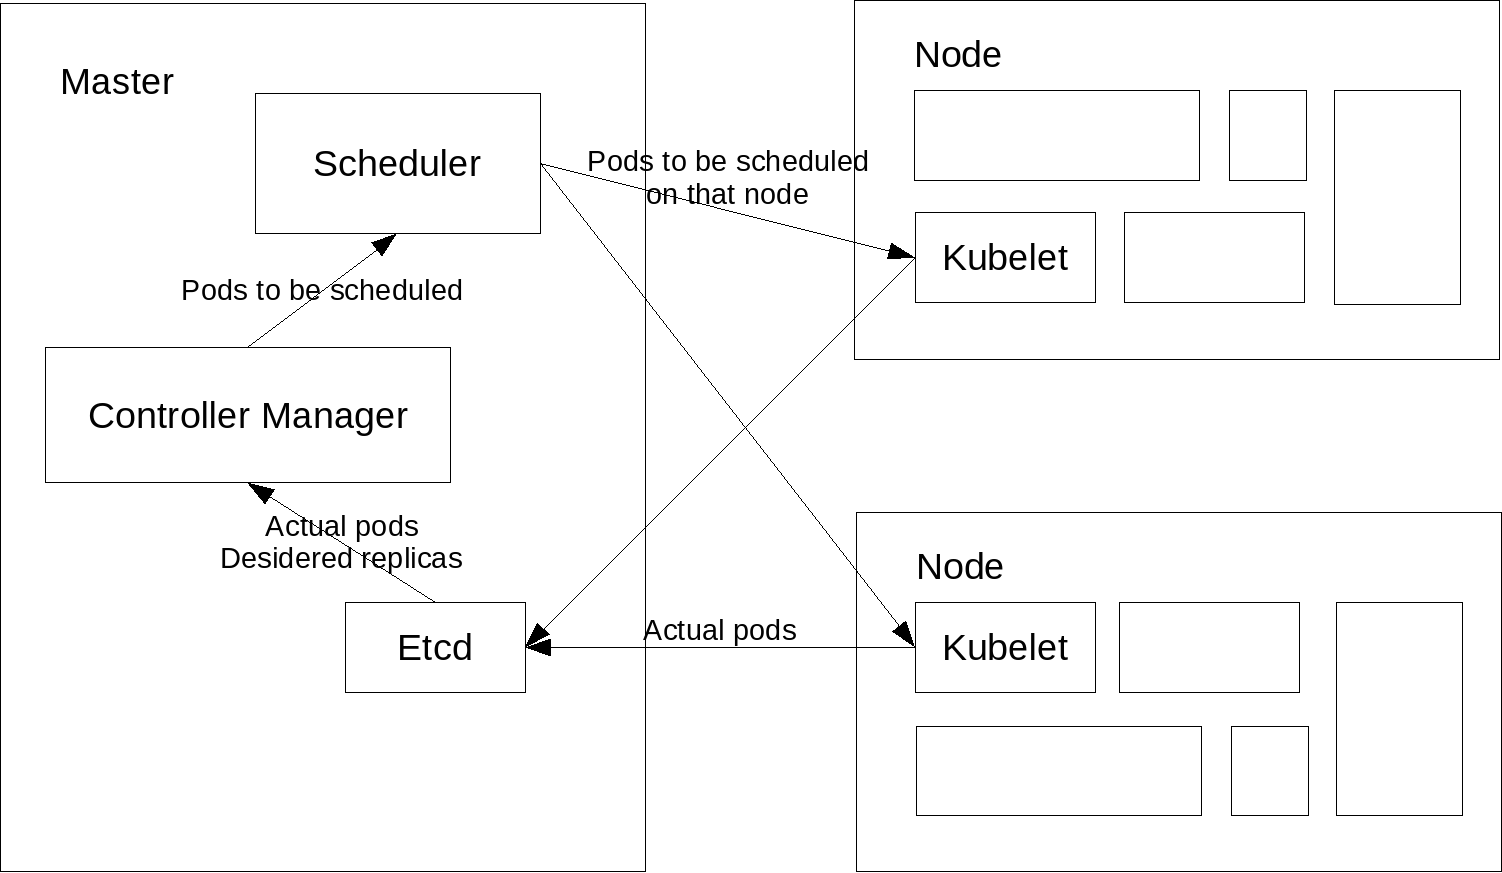
\includegraphics{media/ch5-scheduling.png}
\caption{Replicas and Scheduling}
\end{figure}

On July 20, 2015 the \emph{Linux Foundation} announced the \emph{Cloud
Native Computing Foundation}\cite{CloudNativeComputingFoundation} in
order to standardize the orchestration of components in a cloud
environment, taking Kubernetes as a starting point.

\section{PaaS for Deploying
Applications}\label{paas-for-deploying-applications}

Kubernetes is a great solution, but lacks the concept of application and
the development workflow, so it's more a tool for system specialists. In
order to reach a PaaS abstration, there is needed another level on top
of Kubernetes.

The 3rd version of \emph{OpenShift} is a PaaS built on top of
Kubernetes, providing a solutions for DevOps workflow in modern
container and microservices world.

First of all, OpenShift comes with built-in external router, based on
HAProxy\cite{HAProxy}:

\begin{quote}
HAProxy is a free, open source high availability solution, providing
load balancing and proxying for TCP and HTTP-based applications by
spreading requests across multiple servers. It is written in C and has a
reputation for being fast and efficient (in terms of processor and
memory usage).

HAProxy is used by a number of high-profile websites including GitHub,
Bitbucket, Stack Overflow, Reddit, Tumblr, and Twitter and is used in
the OpsWorks product from Amazon Web Services.
\end{quote}

In order to responding to DNS queries for services, OpenShift includes
\emph{skydns} server.

OpenShift extends Kubernets APIs with additional objects:

\begin{itemize}
\itemsep1pt\parskip0pt\parsep0pt
\item
  \texttt{template} is the building block for applications. Since
  Kubernetes has only conpect of services and not of application,
  template provides a way to define an application as a set components,
  as happens in Docker Compose
\item
  \texttt{route} is configure the HAProxy-based external \texttt{router}
  for external reachability, and point to a \texttt{service}.
\end{itemize}

Future Development will include the following objects in order to enable
Continuous Delivery:

\begin{itemize}
\itemsep1pt\parskip0pt\parsep0pt
\item
  \texttt{build} is the process of creating Docker images from scratch
  or other images
\item
  \texttt{imageStream} represent an image storaged in a repository
\item
  \texttt{deploymentConfig} extends \texttt{replicationController}
  enabling rolling updates in response to signals
\end{itemize}

OpenShift stores the own objects in etcd under \texttt{/openshift.io}
key.

These concepts could be summarized in the following diagram:

\begin{figure}[htbp]
\centering
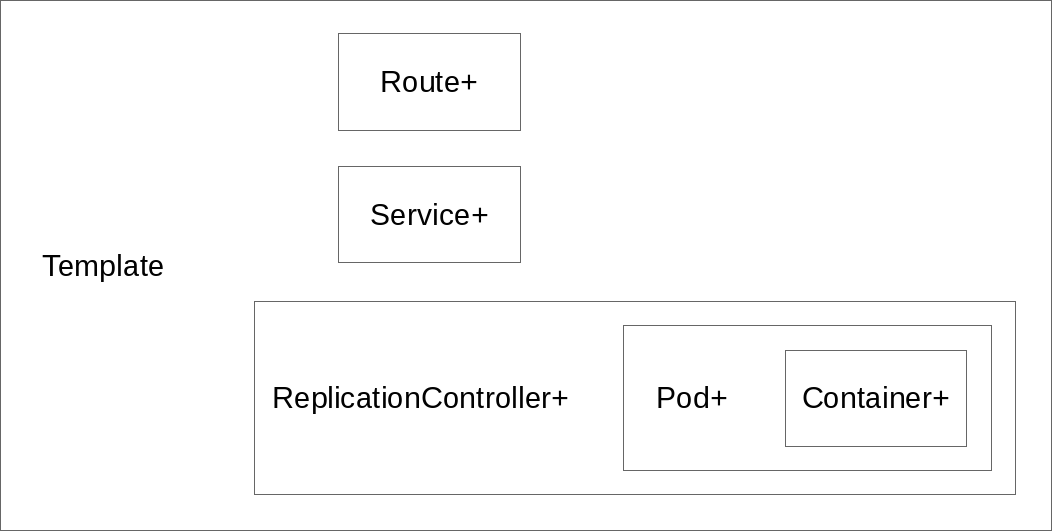
\includegraphics{media/ch5-template.png}
\caption{Route and Template objects}
\end{figure}

Gasista Felice consist of a \texttt{template} that includes a
\texttt{replicationController}/\texttt{service} for every container,
plus a \texttt{route}.

\begin{figure}[htbp]
\centering
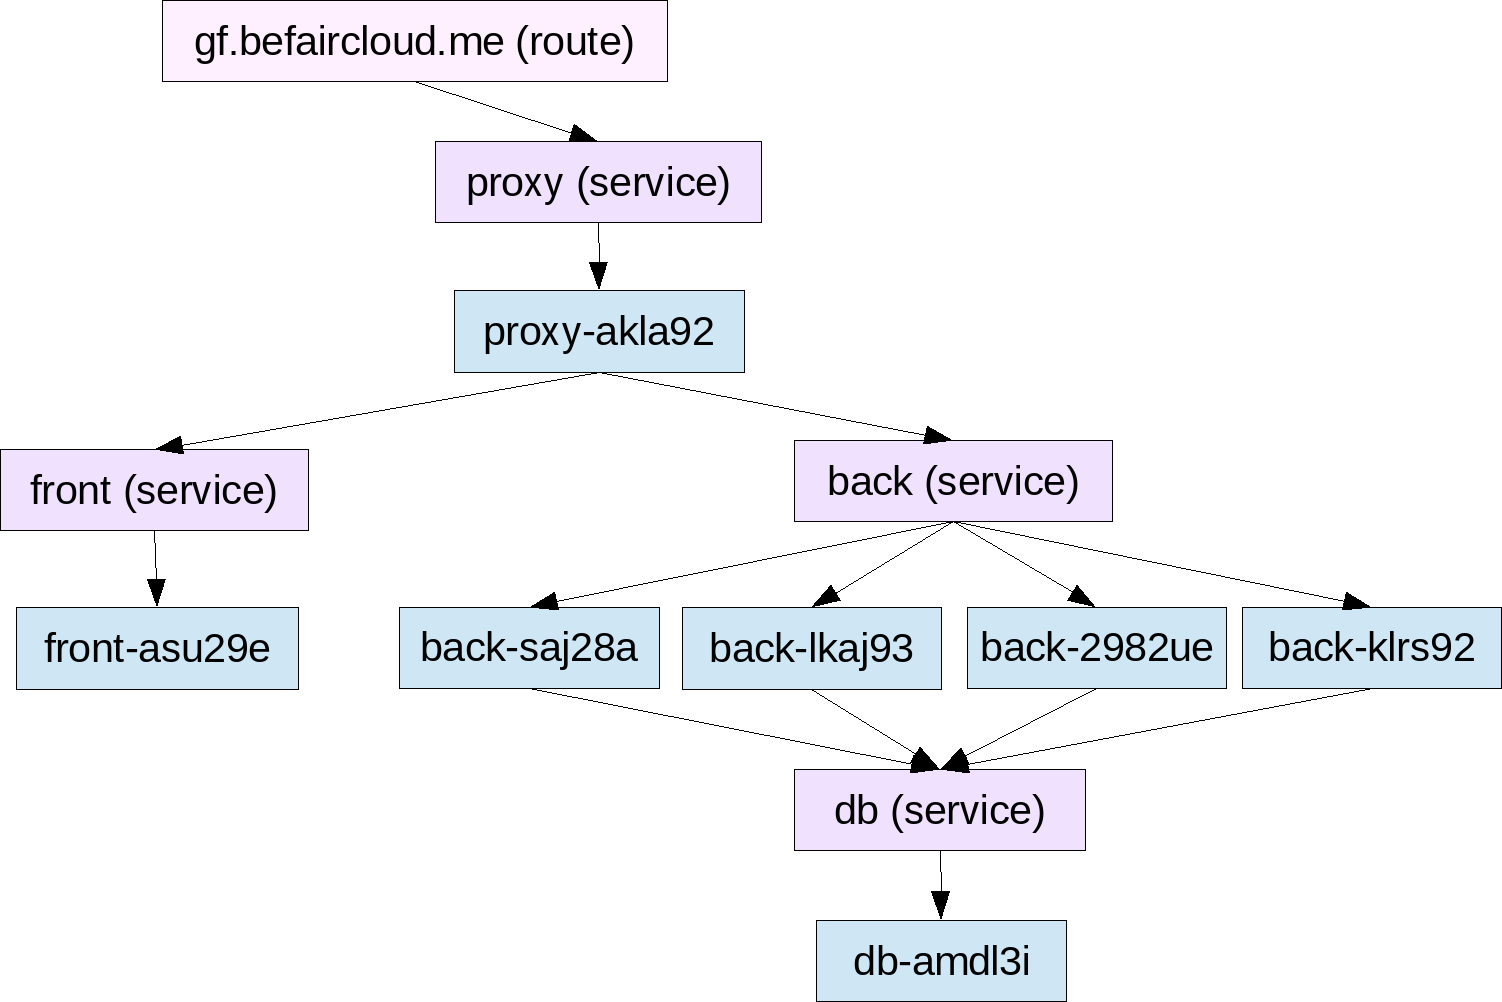
\includegraphics{media/ch5-template-gf.png}
\caption{Gasista Felice template}
\end{figure}

In details:

\begin{itemize}
\itemsep1pt\parskip0pt\parsep0pt
\item
  \emph{database}: while in development the default
  \texttt{postgresql:9.4} image worked fine, on OpenShift it had some
  problems probably due to permissions. So it has been used a dedicated
  image for OpenShift, providing PostgreSQL 9.2, also compatible with
  Gasista Felice. As of other RDBMS, PostgreSQL by design is composed by
  a unique master, and for major scalability in reads, could be setted
  up some slaves but it's not needed.
\item
  The \emph{backend} is the component of uWSGI, Python and Django is the
  main one on which it's possible act. At the end of chapter will be
  provided some benchmarks.
\item
  The \emph{frontend} is mainly useful in development, but in production
  once it has generated the files, it could be cached from NGiNX. In
  further optimization, this component will be deleted at all, and the
  static files will be served directly. In this case will be use
  \texttt{1} replica since there is no need of scaling this component.
\item
  \emph{Proxy} component, NGiNX represent the entry point of the
  application, so it manages caching of static content, demanding to the
  \texttt{front} and \texttt{back} non-cached requests. Since NGiNX is
  generally enough fast thanks to asynchronous loops, should not be
  necessary adding further pods.
\end{itemize}

\section{Benchmarks}\label{benchmarks}

One of the goal of this project is analyze the component for
scalability. Kubernetes's provide the horizontal scaling of pods, so has
been done some benchmarks varying the number of pods of Gasista Felice
backend.

The test consists in using \emph{boom} for 100 concurrent requests for a
total of 100 requests, that consist in a \emph{GET} at
\texttt{/gasistafelice} path of the application, so a
\texttt{GET\ http://gf.befaircloud.me/gasistafelice} in this case. Even
if this should be a simple request, instead involves several work and
represent a simple but significant test case. The values registered
consist in:

\begin{itemize}
\itemsep1pt\parskip0pt\parsep0pt
\item
  \emph{total time}: interval from the beginning of the first request,
  to the end of the last requests
\item
  \emph{requests per second}: represent the medium of requests served
  per second
\end{itemize}

\begin{longtable}[c]{@{}lll@{}}
\caption{Benchmark results}\tabularnewline
\toprule
Backend pods & total time & reqs/s\tabularnewline
\midrule
\endfirsthead
\toprule
Backend pods & total time & reqs/s\tabularnewline
\midrule
\endhead
1 & 34s & 2.5reqs/s\tabularnewline
2 & 33s & 2.7reqs/s\tabularnewline
3 & 26s & 3.7reqs/s\tabularnewline
4 & 20s & 4.8reqs/s\tabularnewline
8 & 22s & 4.5reqs/s\tabularnewline
\bottomrule
\end{longtable}

The results the decreasing time with adding additional pods, to 4 pods.
Beyond 4 pods there is no advantage, probably because of cluster
resource limit.